\chapter{Caking}\label{Caking}

\section{The Caking Algorithm}

A caked plot is similar to a radial ($r$ vs. $\theta$) plot 
of the diffraction data as it would appear if it were
captured on an untilted detector. A radial plot will turn
circles of constant $r$ into straight lines.
Caking is important because diffraction peaks will 
also become straight lines. A caked plot is actually a 
plot of $Q$ vs. $\chi$. Equation \ref{qterms2theta} shows
that $Q$ is related by the $\sin$ function to 
$2\theta$. From equation~\ref{2thetatermsr},
$2\theta$ is related to the radius $r$ by the tangent function.
Although the relationship is not linear, $Q$ increase as $r$ 
increases and therefore $Q$ is similar to $r$.
$\chi$ corresponds to the angle radially around x-ray
beam. So a cake of $Q$ vs. $\chi$ is analogous to a radial 
plot.

Cakes are calculated as follows.
$Q$ and $\chi$ space is first binned. Since each bin has 
some particular $Q$ and $\chi$ value\footnote{Technically,
each bin has a $Q$ and $\chi$ range. The middle of the bin 
is taken to be the particular $Q$ and $\chi$ value.} 
the corresponding $(x''',y''')$ pair can be calculate for each
bin using equation~\ref{invertx} and \ref{inverty}. The
intensity value at the pixel coordinate $(x''',y''')$
is put into the bin.
$(x''',y''')$ is generally between a pixel coordinate so
a bilinear interpolation of the intensity is used to
get a best estimate.

Pixel masks can be used to ignore parts of the caked data.
Whenever the program finds an intensity value
that should be masked (either because it is too 
large, too small, or in a polygon mask), it fills
that part of the caked array with a particular 
negative value. When the caked data is displayed,
these negative values shown with special colors.

The program can perform a polarization correction of
the caked data. The polarization 
correction is
\begin{align}
    I&=Im/PF \\ 
    PF&=P(1 - (\sin(2\theta)\sin(\chi-90))^2) + 
    (1 - P)(1 - (\sin(2\theta)\cos(\chi-90))^2)
\end{align}
with $Im$ the measured intensity. The $2\theta$ and $\chi$
values are for to the particular value that is being 
corrected. All pixels have their 
intensity corrected by this formula before they
are binned.

\section{Caking With the Program}

Caking is done on the \gui{Caking} tab shown in figure~\ref{caking_tab}
The program can only cake data after diffraction data and calibration
parameters have been loaded into the program.
In order to cake, this program needs to know the range
in $Q$ and $\chi$ space that should be caked. 
This can be specified with the \gui{Q Lower?}, \gui{Q Upper?}
\gui{Chi Lower?}, and \gui{Chi Upper?} inputs.
The program also needs to know how many $Q$ and $\chi$ bins to 
create when caking data. This can be set
with the \gui{Number of Q?} and \gui{Number of Chi?} inputs.
The \gui{Do Cake} button can then be used to cake the data. 

\begin{SCfigure}[1][bthp]
    \centering
    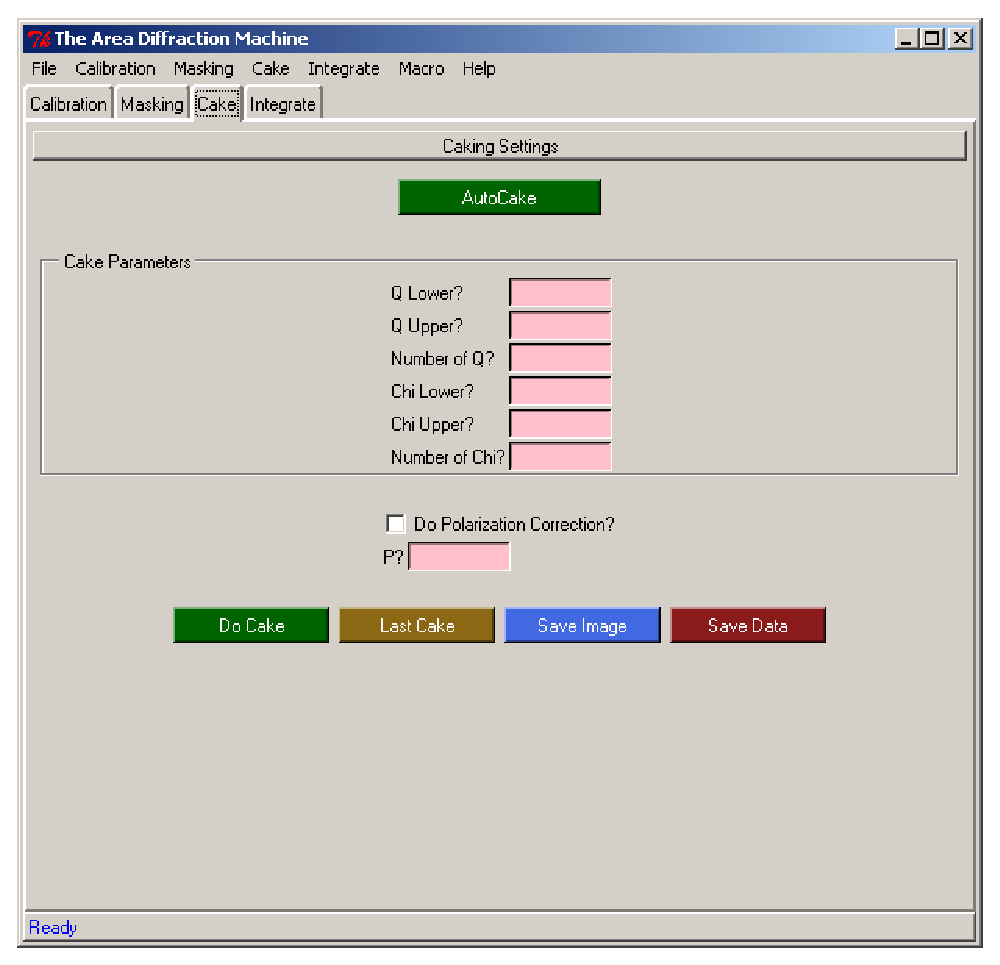
\includegraphics[scale=.75]{figures/caking_tab.eps}
    \caption{Caking is done on the \gui{Caking} tab.} 
    \label{caking_tab}
\end{SCfigure}

\begin{SCfigure}[1][bthp]
    \centering
    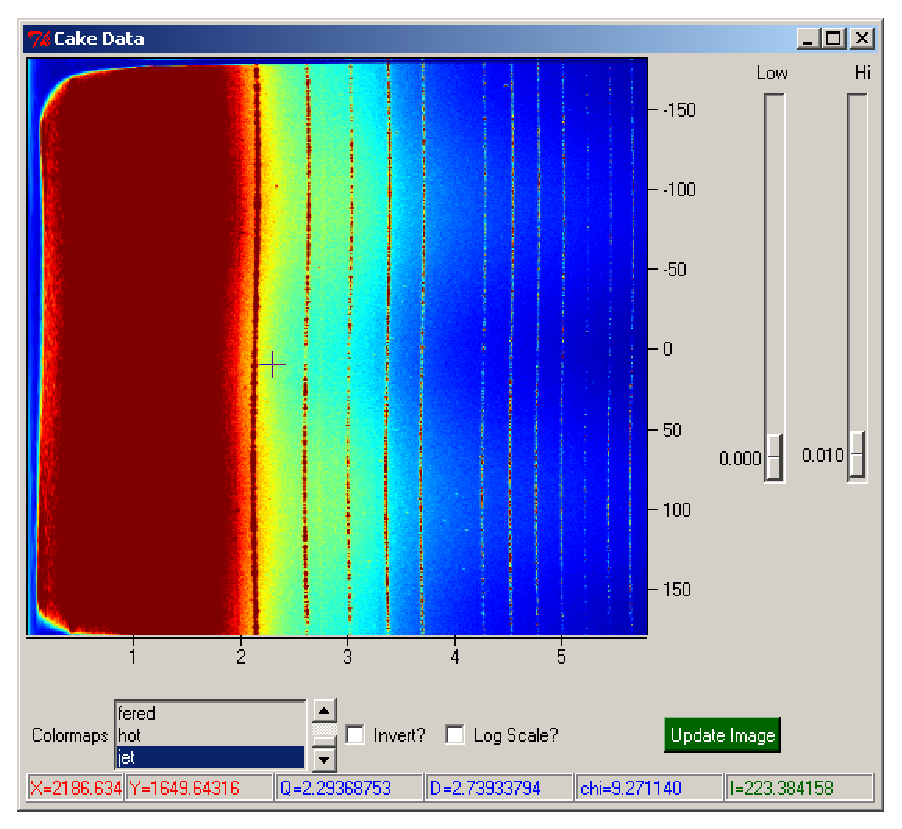
\includegraphics[scale=.75]{figures/cake_data_window.eps}
    \caption{The caked data window will open after the
    data is caked.} 
    \label{cake_data_window}
\end{SCfigure}

After the cake finishes, the program will open a caked data
window that displays the cake data interactively.
The caked data window acts just like the diffraction
data window so everything in Chapter~\ref{viewing_data} 
carries over. The only difference is that whenever
the caked data is zoomed into, the program will take
the selected zoom range and put it into the inputs on
the cake tab and then recake the image. The caked 
can be taken to the previous zoom range with the 
\gui{Last Cake} button 

\section{AutoCake}

\gui{AutoCake} is a button to the \gui{Cake} tab that 
will guess a good range of $Q$ and $\chi$ 
values, put them into the input, and then push the 
\gui{Do Cake} button automatically. It can be used to
create a cake without much work. The program will pick a range
that puts the entire diffraction image into the cake. It will pick
the bins sizes so that each displayed pixel correspond to one bin. 
This will ensure that the cake looks as sharp as the computer 
can display it.

\section{\texorpdfstring{Displaying $Q$ and $\Delta Q$ Lines}
    {Displaying Q and delta Q Lines}}
    \label{cakeQlinesandpeaks}

If a $Q$ list has been loaded into the program, 
constant $Q$ lines or $\Delta Q$ lines can be 
displayed on top of the cake data. Remember that 
constant $Q$ lines on the diffraction image are straight
vertical lines on the caked plot. 
The program will display constant $Q$ lines or 
$\Delta Q$ lines on the caked plot whenever they 
should be displayed on the diffraction image. See 
section~\ref{displayconstQlines} and 
section~\ref{displayconstdQlines} for a discussion of 
displaying constant $Q$ lines on diffraction data.
Figure~\ref{constant_q_lines_on_cake_image} shows constant
$Q$ lines displayed on a caked plot and 
figure~\ref{constant_dq_lines_on_cake_image} shows constant
$\Delta Q$ lines displayed on a caked plot.


\begin{figure}[bthp]
    \centering
    \subfloat[A cake with constant $Q$ 
    lines drawn on top of it.]{
    \label{constant_q_lines_on_cake_image}
    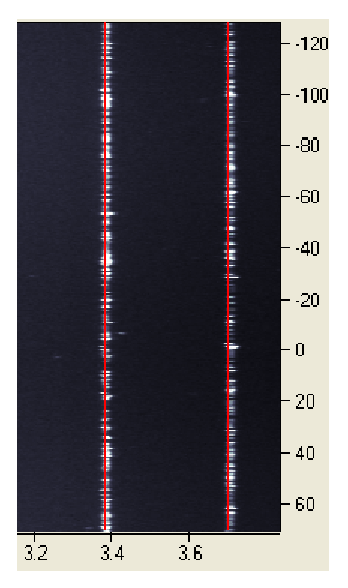
\includegraphics[scale=.75]
    {figures/constant_q_lines_on_cake_image.eps}}\hspace{1em}
    \subfloat[A cake with constant $\Delta Q$ 
    lines drawn on top of it.]{
    \label{constant_dq_lines_on_cake_image}
    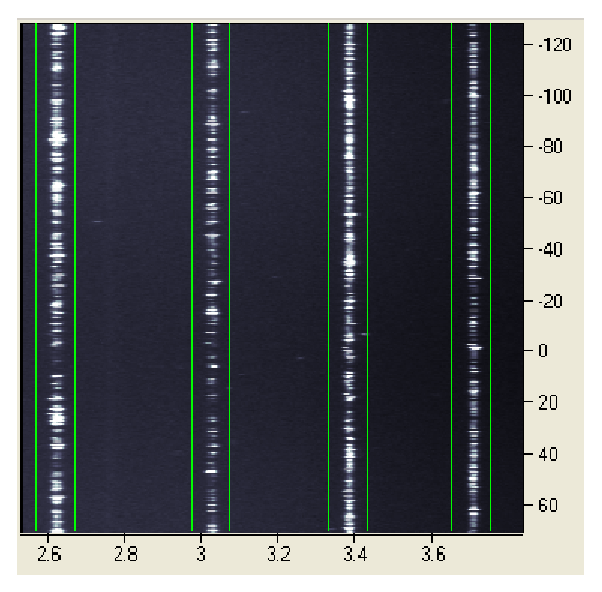
\includegraphics[scale=.75]
    {figures/constant_dq_lines_on_cake_image.eps}}\hspace{1em}
    \subfloat[A cake with diffraction peaks drawn on top of it.]{
    \label{peaks_on_cake_image}
    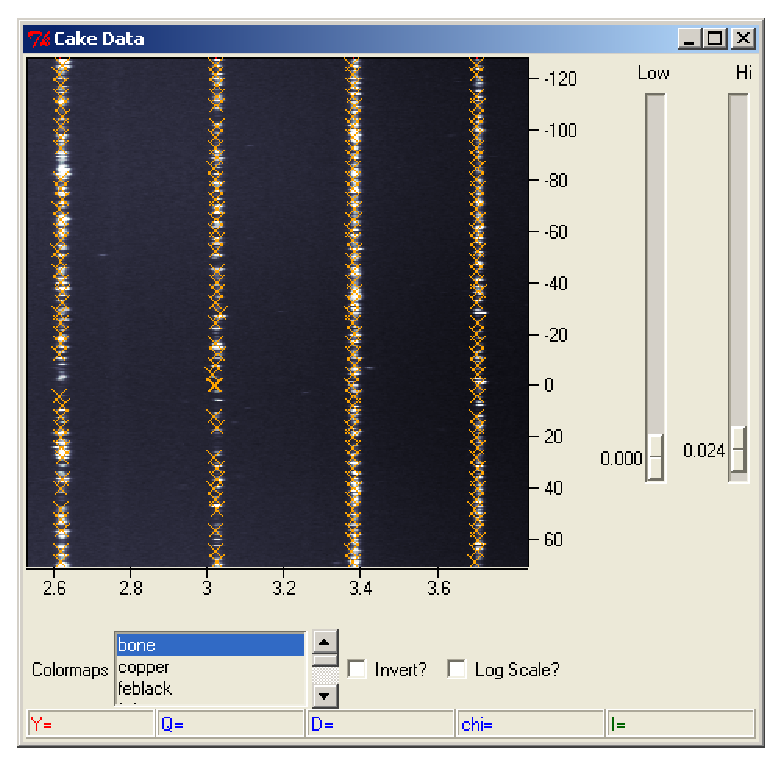
\includegraphics[scale=.75]{figures/peaks_on_cake_image.eps}}
    \label{calibration_cake}
\end{figure}

\section{Displaying Peaks}\label{displaying_peaks_cake}

Any peaks that the program finds when performing
a calibration can be displayed on top of the caked
data as crosses. Peaks will be displayed on the caked plot whenever 
they are displayed on the diffraction image. 
Figure~\ref{peaks_on_cake_image} 
shows peaks displayed on a caked plot.  Being able to display 
$Q$ lines and peaks on caked data can be very useful for 
checking if the calibration was done properly. 
Figure~\ref{calibration_cake} illustrates this principle.

\begin{figure}[htb]
    \centering
    \subfloat[A bad calibration]{
    \label{bad_calibration_cake_zoom_peaks}
    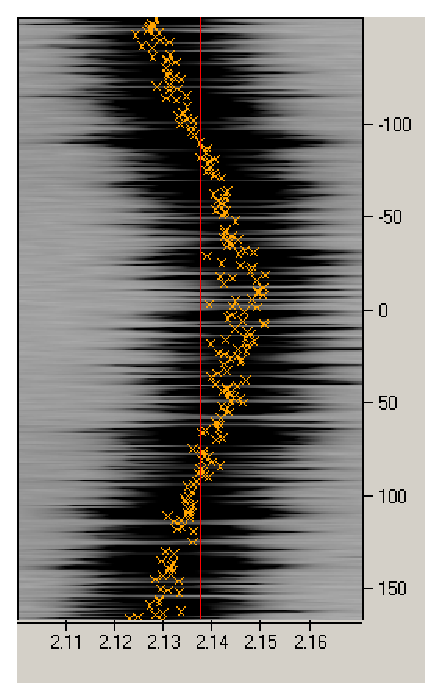
\includegraphics[scale=.75]{figures/bad_calibration_cake_zoom_peaks.eps}}\hspace{1em}
    \subfloat[A good calibration]{
    \label{good_calibration_cake_zoom_peaks}
    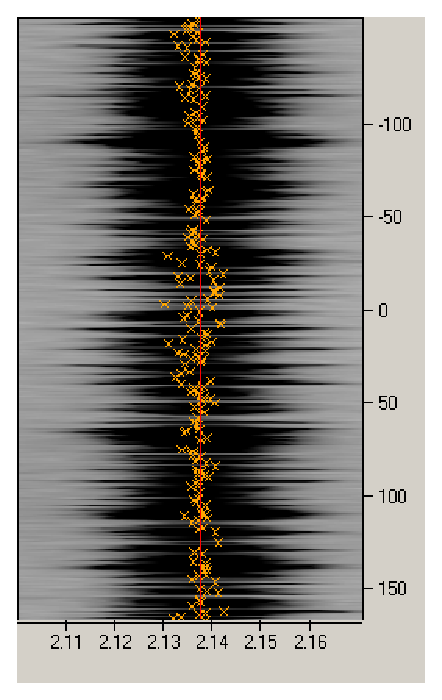
\includegraphics[scale=.75]{figures/good_calibration_cake_zoom_peaks.eps}}		
    \caption{Displaying peaks and constant $Q$ lines on top of a 
    cake of a standard crystal can be used to tell if the data is properly 
    calibrated. If the calibration is bad, the diffraction peaks will have 
    a systematic distortion. If the calibration is good, all the peaks will 
    cluster very close to their particular $Q$ value and there will be no 
    systematic distortion. This can be used to see if the program is properly 
    calibrating diffraction data.}
    \label{calibration_cake_zoom}
\end{figure}

\section{Polarization Correction}
The program can apply a polarization correction to the
cake. The \gui{Do Polarization Correction?} check box
can be used to apply a polarization and the 
polarization value can be set with the \gui{P?} input.

\section{\texorpdfstring{Working in $2\theta$}{Working in 2theta}}

Caked plots can have $2\theta$ instead of $Q$ as one
of the axes.  This can be done by changing the program
to $2\theta$ mode by doing into the file menu and selecting 
the \gui{Work in 2theta} option. When this is selected,
all the names in the program will change from $Q$ to $2\theta$. 
The program will have \gui{$2\theta$ Lower}, \gui{$2\theta$ Upper}, 
and \gui{Number of $2\theta$} as inputs. The allowed range will
then be in $2\theta$ and the program will display the cake image with
$2\theta$ as its axis. The corresponding \gui{Work in Q} option 
can be used to return the program to caking in $Q$.
This feature was introduces in version 2.0.0 of the program.

\section{Saving Cake Data}

Caked data can also be saved as a plain text data file
using the \gui{Save Data} button. The format for cake files is 
a long comment string followed by the data in rows of numbers:
\begin{lstlisting}[caption={'caked\_data.dat'}]
# Cake of: N:/data/LaB6_14_02_56.mar3450 
# Data Caked on Wed Mar 12 21:30:55 2008
# Calibration data used to make the cake:
#   x center:    1725.0000000 pixels
#   y center:    1725.0000000 pixels
#   distance:     125.2960000 mm
#   energy:     12735.3957721 eV
#   alpha:          0.0000000 degrees
#   beta:           0.0000000 degrees
#   rotation:       0.0000000 degrees
#   pixel length:     100.0000000 microns
#   pixel height:     100.0000000 microns
# A Polarization correction was applied
#   P = 0.500000
# A greater than mask was applied
#   Greater than mask = 1000.000000
# A Less Than Mask was applied
#   Less than mask = 10.000000
# Polygon mask(s) were applied
# Polygon(s) used in the analysis:
#   2400.10912343	1073.5706619
#   962.511627907	2282.88014311
#   2850.51520572	2572.86762075
#
#   1573.33631485	1215.47942755
#   1820.13416816	2893.70483005
#   2906.04472272	1573.33631485
# Cake range:
#   Q Lower = 0.000000
#   Q Upper = 6.726544
#   Number of Q = 560.000000
#   Q Step = 0.012012
#   chi Lower = -180.000000
#   chi Upper = 180.000000
#   Number of Chi = 560.000000
#   chi Step = 0.642857
# Note: pixels outside the diffraction image are saved as -1
#   Pixels greater than the greater than mask are saved as -2
#   Pixels less than the less than mask are saved as -3
#   Pixels inside of a polygon masks are saved as -4
# chi increased down. Q increases to the right
\end{lstlisting}
the comment string describes what state the program was in when the 
cake was done. It first lists the name of the diffraction 
file(s) that were caked. It then lists the calibration parameters 
used when caking the data. It then lists the polarization correction, 
the greater than mask and the less than mask that were used. It then lists 
the pixel 
coordinates of any polygons that were used when caking.  It then lists 
the range of the cake and the number of bins that were used.
The program tries to be smart about the comment string. If no 
masks were used, the comment string would instead contains 
\begin{lstlisting}[caption={'Alternate Header'}]
# No greater than mask was applied
# No less than mask was applied
# No polygon masks were applied
\end{lstlisting}
If the program is working in $2\theta$ mode, the comment string will 
instead say something like
\begin{lstlisting}[caption={'Another Alternate Header'}]
#   2theta Lower = 0.000000
#   2theta Upper = 62.814525
#   number of 2theta = 560.000000
#   2theta Step = 0.112169
\end{lstlisting}

Next in the file is the data. Each line in the file is of constant 
$\chi$ and contains many numbers separated by
spaces. Each column is of constant $Q$. $\chi$ increases down and 
$Q$ increases to the right. The program sets certain bins in 
in the data to special values. Bins that are outside the diffraction
image are saved as -1. Bins that are masked because they were too 
large are saved as -2. Bins that are masked because they were too 
small are saved as -3. Bins that are inside a pixel mask are saved 
as -4. This is also put in the comment string. 


\section{Saving Cake Images}

Caked data can be saved as one of many popular image formats.
The program can save caked images as \gui{jpg}, \gui{gif}, \gui{eps}, 
\gui{pdf}, \gui{bmp}, \gui{png}, or \gui{tiff}.  A caked image
will be saved with whatever threshold masks, polygon masks, $Q$ lines, 
$\Delta Q$ lines, and peaks were displayed over the caked data. 


